\documentclass[12pt,a4paper]{article}

% ─── 1. PACKAGES ──────────────────────────────────────────────────────────────
\usepackage[utf8]{inputenc}
\usepackage[T1]{fontenc}
\usepackage{amsmath, amssymb}
\usepackage{geometry}
\usepackage{graphicx}
\usepackage{xcolor}
\usepackage{listings}
\usepackage{hyperref}
\usepackage{booktabs}
\usepackage{enumitem}
\usepackage{tcolorbox}
\usepackage{mdframed}
\usepackage{fancyhdr}
\usepackage{titlesec}
\usepackage{tikz} 
\usetikzlibrary{shapes.geometric, positioning, arrows.meta, calc, trees}

% Font Settings
\usepackage{newtxtext,newtxmath} % Times New Roman
\usepackage{courier}             % Courier New untuk kode

\geometry{margin=2.5cm}

% ─── 2. WARNA TEMA ────────────────────────────────────────────────────────────
\definecolor{codebg}{RGB}{245,247,250}
\definecolor{codeframe}{RGB}{180,195,215}
\definecolor{keywordcolor}{RGB}{0,112,192}
\definecolor{commentcolor}{RGB}{100,160,100}
\definecolor{stringcolor}{RGB}{180,70,50}
\definecolor{notebg}{RGB}{255,249,230}
\definecolor{noteframe}{RGB}{230,180,50}
\definecolor{tipbg}{RGB}{230,245,235}
\definecolor{tipframe}{RGB}{50,160,90}
\definecolor{sectioncolor}{RGB}{30,80,150}

% ─── 3. STYLE SECTION & TOC ───────────────────────────────────────────────────
\titleformat{\section}{\Large\bfseries\color{sectioncolor}}{}{0em}{\thesection\quad}[\titlerule]
\titleformat{\subsection}{\large\bfseries\color{sectioncolor!80}}{}{0em}{\thesubsection\quad}

% Style Table of Contents
\usepackage{tocloft}
\renewcommand{\cftsecleader}{\cftdotfill{\cftdotsep}}
\renewcommand{\cftsecfont}{\bfseries\color{sectioncolor}}

% ─── 4. LISTINGS (CODE STYLE) ─────────────────────────────────────────────────
\lstdefinestyle{customstyle}{
  basicstyle=\ttfamily\small,
  backgroundcolor=\color{codebg},
  frame=single,
  rulecolor=\color{codeframe},
  keywordstyle=\bfseries\color{keywordcolor},
  commentstyle=\itshape\color{commentcolor},
  stringstyle=\color{stringcolor},
  numbers=left,
  numberstyle=\tiny\color{gray},
  breaklines=true,
  tabsize=4,
  showstringspaces=false
}
\lstset{style=customstyle}

% ─── 5. KOTAK CATATAN (MD-FRAME) ──────────────────────────────────────────────
\newmdenv[
  backgroundcolor=notebg, linecolor=noteframe, linewidth=2pt,
  leftline=true, topline=false, rightline=false, bottomline=false,
  innerleftmargin=10pt, innertopmargin=6pt, innerbottommargin=6pt, skipabove=8pt
]{notebox}

\newmdenv[
  backgroundcolor=tipbg, linecolor=tipframe, linewidth=2pt,
  leftline=true, topline=false, rightline=false, bottomline=false,
  innerleftmargin=10pt, innertopmargin=6pt, innerbottommargin=6pt, skipabove=8pt
]{tipbox}

% ─── 6. HEADER & FOOTER ───────────────────────────────────────────────────────
\pagestyle{fancy}
\fancyhf{}
\fancyhead[L]{\small\textit{Rekayasa Perangkat Lunak}}
\fancyhead[R]{\small\textit{noteify -- Pemodelan PL}}
\fancyfoot[C]{\thepage}
\renewcommand{\headrulewidth}{0.4pt}

% ─── 7. DATA COVER ────────────────────────────────────────────────────────────
\title{
  {\LARGE\bfseries REKAYASA PERANGKAT LUNAK}\\[0.5em]
  {\large Modul Pembelajaran: Pemodelan Perangkat Lunak dan UML}\\[0.8em]
  {\normalsize Penjelasan komprehensif mengenai konsep representasi sistem, landasan metodologi berorientasi objek, serta standar visualisasi diagram UML.}
}
\author{}
\date{}

% ==============================================================================
\begin{document}

\maketitle
\thispagestyle{fancy}
\tableofcontents
\newpage

% ─── KONTEN MATERI ─────────────────────────────────────────────────────────────

\section{Pemahaman Dasar Pemodelan Sistem}

Sebelum menulis baris kode program, seorang \textit{Software Engineer} harus mampu merancang cetak biru (\textit{blueprint}) dari sistem yang akan dibangun. Proses perancangan ini disebut dengan \textbf{pemodelan}.

Secara definisi, \textbf{Pemodelan (Model)} adalah representasi dari sebuah sistem nyata yang telah disederhanakan. Tujuannya agar kompleksitas sistem dapat lebih mudah dipelajari, dipahami, dan dikomunikasikan antar anggota tim. Dengan menggunakan model, tim pengembang dapat melakukan visualisasi, spesifikasi, konstruksi, dan dokumentasi secara lebih terstruktur sebelum sistem diimplementasikan dalam bentuk kode.

Ada 5 macam gaya atau cara merepresentasikan sebuah model sistem:

\begin{enumerate}
    \item \textbf{Physical (Fisik):} Membuat versi nyata dengan skala yang diperkecil (\textit{scaled-down version}) dari sistem yang dipelajari. Contohnya: miniatur model pesawat, model kereta api, atau prototipe hardware yang mendemonstrasikan aspek fungsional dari sistem sebenarnya.
    
    \item \textbf{Pictorial (Gambar):} Representasi menggunakan lukisan atau gambar untuk mendeskripsikan suatu bidang atau fenomena. Contohnya: peta topografi kontur bumi, bola dunia (globe), atau diagram aliran air dalam sistem hidrologi.
    
    \item \textbf{Verbal:} Representasi suatu sistem menggunakan susunan kata dan kalimat verbal yang mendeskripsikan ukuran, bentuk, dan karakteristik sistem tersebut. Pendekatan ini bermanfaat untuk dokumentasi requirements dan spesifikasi kebutuhan yang ditulis dalam bentuk narasi atau daftar kebutuhan.
    
    \item \textbf{Schematic (Skema):} Representasi dalam bentuk skema figuratif yang menggabungkan simbol-simbol dengan garis penghubung. Contohnya: skema rangkaian listrik, skema alur proses produksi, atau model atom Bohr dalam kimia.
    
    \item \textbf{Symbolic (Simbolik):} Representasi ke dalam bentuk simbol-simbol matematika, di mana karakteristik variabel diformulasikan menggunakan persamaan matematika. Pendekatan ini sangat berguna untuk sistem yang memiliki perilaku kuantitatif atau algoritma kompleks yang dapat diekspresikan secara matematis.
\end{enumerate}

\subsection{Karakteristik Kualitas Proses Pemodelan Analisis}

Saat melakukan proses pemodelan analisis, kita harus mengevaluasi apakah proses yang kita jalankan sudah baik atau belum. Evaluasi ini penting untuk memastikan bahwa model yang dihasilkan dapat digunakan secara efektif oleh seluruh tim pengembang. Ada 8 indikator kualitas proses analisis yang perlu dipertimbangkan:

\begin{itemize}
    \item \textbf{Understandability (Kemudahan Pemahaman):} Sejauh mana proses didefinisikan secara eksplisit dan seberapa mudah definisi proses itu dipahami oleh anggota tim. Model yang baik harus dapat dipahami oleh semua stakeholder tanpa memerlukan penjelasan yang berbelit-belit.
    
    \item \textbf{Visibility (Visibilitas):} Apakah aktivitas proses menghasilkan titik akhir (keluaran) yang jelas, sehingga kemajuan dari proses tersebut terlihat nyata. Setiap tahap harus menghasilkan deliverable yang terukur dan dapat diverifikasi.
    
    \item \textbf{Supportability (Dukungan Alat):} Sejauh mana aktivitas proses dapat didukung oleh alat bantu CASE (\textit{Computer-Aided Software Engineering}). Alat seperti ArchiMate, Enterprise Architect, atau Lucidchart dapat mempercepat proses pemodelan.
    
    \item \textbf{Acceptability (Penerimaan):} Apakah proses yang telah ditentukan dapat diterima, digunakan, dan dipertanggungjawabkan selama pembuatan perangkat lunak. Proses harus selaras dengan budaya organisasi dan tidak menimbulkan resistensi dari tim.
    
    \item \textbf{Reliability (Keandalan):} Apakah proses didesain sedemikian rupa sehingga \textit{error} (kesalahan) proses dapat dihindari sebelum merusak produk akhir. Mekanisme quality assurance dan review harus tertanam dalam proses.
    
    \item \textbf{Robustness (Ketangguhan):} Dapatkah proses pengembangan terus berjalan walaupun terjadi masalah \textit{error} yang tidak diduga di tengah jalan. Proses yang robust memiliki mekanisme fallback dan recovery yang baik.
    
    \item \textbf{Maintainability (Kemudahan Pemeliharaan):} Dapatkah proses berkembang dan beradaptasi untuk mengikuti perubahan kebutuhan atau perbaikan. Model dan proses harus mudah diperbarui tanpa memerlukan rekonstruksi total.
    
    \item \textbf{Rapidity (Kecepatan):} Bagaimana tingkat kecepatan proses untuk dapat memenuhi seluruh spesifikasi yang diminta secara lengkap. Proses yang baik harus efisien dalam hal waktu dan sumber daya tanpa mengorbankan kualitas.
\end{itemize}

\newpage
\section{Landskap Metodologi Analisis}

Secara garis besar, pendekatan pemodelan analisis terbagi menjadi dua mazhab besar: \textbf{Analisis Terstruktur} (klasik) dan \textbf{Analisis Berorientasi Objek} (modern). Analisis Terstruktur menggunakan pendekatan \textit{top-down} yang memecah sistem menjadi komponen-komponen data dan proses yang lebih kecil. Sebaliknya, Analisis Berorientasi Objek menggabungkan data dan perilaku ke dalam entitas yang disebut objek.

Pada modul ini, kita akan berfokus pada Metodologi Berorientasi Objek (\textit{Object-Oriented}). Sebelum standar UML diresmikan pada tahun 1997, ada banyak pakar yang menciptakan metode \textit{Object-Oriented} (OO) mereka sendiri dengan notasi dan terminologi yang berbeda-beda. Berikut adalah 6 metode OO paling bersejarah yang akhirnya melebur menjadi UML:

\begin{enumerate}
    \item \textbf{Metode Booch (Object Oriented Design)}\\
    Metode ini dikembangkan oleh Grady Booch dan membagi proses analisis dan desain ke dalam 4 tahapan iteratif (berulang): 
    \begin{enumerate}[label=(\arabic*)]
        \item Identifikasi kelas dan objek dari domain masalah
        \item Identifikasi semantik dan hubungan antar objek
        \item Perincian \textit{interface} (antarmuka) dan implementasi
        \item Dokumentasi dan verifikasi
    \end{enumerate}
    Metode ini terkenal dengan diagram object-oriented yang detail dan notation yang comprehensive.
    
    \item \textbf{Metode Rumbaugh (Object Modelling Technique - OMT)}\\
    Berdasarkan pada analisis terstruktur dan pemodelan \textit{Entity Relationship} (ER). Memiliki 3 tahap utama: 
    \begin{enumerate}[label=(\arabic*)]
        \item Analisis Object Model, Dynamic Model, dan Functional Model
        \item Desain Sistem dan desain Object-oriented
        \item Implementasi dan pengujian
    \end{enumerate}
    Keunggulannya adalah memiliki notasi yang mendukung semua konsep OO dan mudah diterapkan oleh tim yang sudah terbiasa dengan ER diagram.
    
    \item \textbf{Metode Jacobson (Object Oriented Software Engineering - OOSE)}\\
    Metode inilah yang menjadi cikal bakal (pioneer) konsep \textit{Use-Case} yang sangat popular hingga saat ini. Tahapannya meliputi: 
    \begin{enumerate}[label=(\arabic*)]
        \item Model \textit{requirement} dan analisis menggunakan use-case
        \item Desain dan implementasi architecture
        \item Model pengujian (test model)
    \end{enumerate}
    Keunggulannya adalah notasinya sangat sederhana, mudah dipelajari, dan sangat efektif untuk komunikasi dengan stakeholder non-teknis.
    
    \item \textbf{Metode Coad dan Yourdon}\\
    Berfokus pada pemodelan OO dan ER dengan 4 komponen perancangan: 
    \begin{enumerate}[label=(\arabic*)]
        \item Problem domain (domain masalah)
        \item Human interaction (interaksi manusia / UI)
        \item Data management (manajemen data / persistence)
        \item Task management (manajemen tugas / workflow)
    \end{enumerate}
    Metode ini sangat aplikatif untuk sistem bisnis yang kompleks.
    
    \item \textbf{Metode Wirfs-Brock (RDD / CRC - Responsibility Driven Design)}\\
    Metode \textit{Responsibility Driven Design} (RDD) ini sangat berguna untuk memunculkan ide di tahap awal analisis. Metode ini menggunakan kartu CRC (\textit{Class Responsibility Collaboration}) untuk mengidentifikasi:
    \begin{enumerate}[label=(\arabic*)]
        \item Kelas dan tanggung jawab (responsibility) masing-masing
        \item Kolaborasi antar kelas
        \item Hierarki pewarisan kelas
    \end{enumerate}
    Pendekatan ini sangat interaktif dan sering digunakan dalam workshop analisis kelompok.
    
    \item \textbf{Metode Shlaer-Mellor (OOA/D Tradisional)}\\
    Menghasilkan tiga jenis model yang saling melengkapi:
    \begin{enumerate}[label=(\arabic*)]
        \item Information model (diagram class/entity)
        \item State model (diagram state/transisi state)
        \item Process model (diagram aksi dan aktivitas)
    \end{enumerate}
    Metode ini sangat mudah dikonversi dari metode struktural lama ke OO, sehingga cocok untuk organisasi yang sedang melakukan transisi dari structured programming ke object-oriented.
\end{enumerate}

\newpage
\section{Pengenalan Unified Modeling Language (UML)}

Karena dulu banyak pakar yang membuat standar diagramnya sendiri-sendiri, masing-masing dengan kelebihan dan kelemahan tersendiri, akhirnya pada pertengahan 1990-an disepakatilah sebuah standar global yang menggabungkan praktik terbaik dari semua metode di atas. Standar tersebut bernama \textbf{Unified Modeling Language (UML)}, yang diresmikan oleh \textit{Object Management Group (OMG)} pada tahun 1997.

UML adalah kumpulan notasi yang lengkap untuk membuat visualisasi model suatu sistem. Notasi-notasi ini bersifat grafis dan memiliki semantik yang jelas, sehingga dapat dipahami oleh berbagai stakeholder. Tujuan utama diciptakannya UML adalah:

\begin{enumerate}
    \item Memberikan bahasa pemodelan visual yang ekspresif, siap pakai, dan mudah dimengerti secara umum agar pengembang dapat saling menukar model dan berkomunikasi dengan efektif.
    
    \item Memberikan standar pemodelan yang independen (bebas dari ikatan bahasa pemrograman tertentu, platform tertentu, atau proses rekayasa tertentu), sehingga UML dapat diterapkan di berbagai konteks dan lingkungan.
    
    \item Menyatukan \textit{best-practices} (praktik-praktik terbaik) yang selama ini digunakan dalam dunia pemodelan sistem, menciptakan satu bahasa bersama untuk industri software engineering.
\end{enumerate}

\subsection{Kategori Diagram dalam UML}

Ada beberapa jenis diagram utama dalam UML yang dapat dikelompokkan berdasarkan fungsinya:

\begin{itemize}
    \item \textbf{Diagram Struktur (Structural Diagrams):} Menggambarkan elemen-elemen statis dalam sistem seperti kelas, objek, komponen, dan hubungan antar mereka. Termasuk: Class Diagram, Object Diagram, Component Diagram, Deployment Diagram, Package Diagram.
    
    \item \textbf{Diagram Perilaku (Behavioral Diagrams):} Menggambarkan aspek dinamis atau perilaku sistem, bagaimana sistem berinteraksi dan bereaksi terhadap events. Termasuk: Use Case Diagram, Sequence Diagram, Activity Diagram, State Machine Diagram, Communication Diagram, Interaction Overview Diagram.
\end{itemize}

Mari kita bahas beberapa diagram utama secara mendetail.

\newpage
\section{1. Use Case Diagram}

\textbf{Use Case Diagram} merupakan sebuah diagram yang bertujuan untuk menggambarkan \textbf{fungsionalitas} (feature atau capability) yang diharapkan dari sebuah sistem. Diagram ini fokus mendeskripsikan interaksi atau hubungan antara \textit{Aktor} (pengguna/pihak luar) dengan \textit{Sistem} itu sendiri melalui sebuah skenario cerita penggunaan (use case).

Use Case Diagram sangat bermanfaat pada tahap awal analisis kebutuhan (\textit{requirements analysis}) karena:
\begin{itemize}
    \item Membantu mengidentifikasi semua pengguna sistem (aktor) dan kebutuhan mereka
    \item Memberikan gambaran high-level tentang apa yang bisa dilakukan sistem
    \item Memfasilitasi komunikasi antara developer dan stakeholder
    \item Menjadi dasar untuk pembuatan test cases dan dokumentasi kebutuhan
\end{itemize}

Ada 6 elemen/komponen pembentuk Use Case Diagram:

\textbf{1. System (Sistem)}\\
Menyatakan batasan (\textit{boundary}) ruang lingkup sistem. Digambarkan dengan kotak segi empat yang membatasi semua use case di dalamnya. Semua aktor harus berada di luar kotak ini. (Catatan: Seringkali kotak batas sistem ini disembunyikan/tidak digambar karena dianggap sudah jelas dari konteks).

\textbf{2. Actor (Aktor)}\\
Aktor adalah entitas di luar sistem yang akan menggunakan atau berinteraksi dengan sistem tersebut. Aktor tidak selalu manusia; ia bisa berupa \textit{device} (perangkat keras seperti sensor, printer) atau bahkan sistem/server lain (seperti database server, payment gateway). Cara mudah mencari aktor adalah dengan bertanya: \textit{``Siapa/apa yang akan menggunakan sistem ini?''} dan \textit{``Apakah sistem ini memberikan nilai/manfaat bagi dia?''} Setiap aktor dalam diagram harus mempunyai setidaknya satu use case.

\textbf{3. Use Case (Fungsionalitas)}\\
Mengidentifikasi fitur atau \textit{goal} (tujuan) utama dari sistem yang dicapai melalui interaksi dengan aktor. Digambarkan dengan bentuk Elips oval dengan nama aktivitas di dalamnya. Setiap use case pasti memiliki pemicu (\textit{trigger}) yang memulainya. \textit{Trigger} bisa bersifat \textbf{eksternal} (misal: user menekan tombol pesan) atau \textbf{temporal/waktu} (misal: alarm berbunyi saat jadwal jatuh tempo).

\textbf{4. Association (Asosiasi)}\\
Garis penghubung yang mengidentifikasi interaksi antara aktor dengan use case tertentu. Bisa berupa garis lurus tanpa panah (interaksi dua arah) atau dengan panah (komunikasi satu arah). Association mewakili partisipasi dari aktor dalam use case tersebut.

\textbf{5. Dependency (Ketergantungan)}\\
Garis putus-putus berpanah yang menunjukkan hubungan ketergantungan antar dua Use Case. Terdiri dari 2 jenis:
\begin{itemize}
    \item \textbf{<<include>> (Inclusion):} Use case yang satu WAJIB memanggil use case yang lain agar bisa selesai dengan sempurna. Hubungan ini bersifat unconditional dan mandatory. (Arah panah menuju ke use case yang dipanggil/included).
    \item \textbf{<<extend>> (Extension):} Pemanggilan use case tambahan HANYA JIKA kondisi tertentu terpenuhi (opsional). Hubungan ini bersifat conditional dan optional. (Arah panah berlawanan, menuju ke use case pemanggil/yang diperluas).
\end{itemize}

\textbf{6. Generalization (Generalisasi)}\\
Mendefinisikan relasi pewarisan sifat (\textit{inheritance}) antar use case atau antar aktor. Digambarkan dengan garis bermata panah kosong (segitiga putih) yang mengarah dari sisi \textit{Child} (anak) ke sisi \textit{Parent} (induk). Ini menunjukkan bahwa aktor child mewarisi semua karakteristik dari parent.

\begin{figure}[h]
    \centering
    \vspace{-0.5cm}
    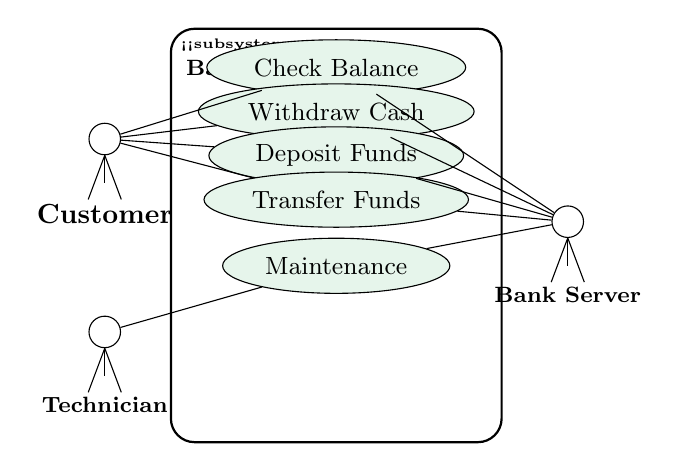
\begin{tikzpicture}[scale=0.7, every node/.style={font=\small}]
    
        % System Boundary
        \draw[thick, rounded corners=0.3cm] (1.5, 3.5) rectangle (7.5, -4);
        \node[anchor=north west, font=\tiny] at (1.5, 3.5) {\textbf{<<subsystem>>}};
        \node[anchor=north west, font=\footnotesize\bfseries] at (1.6, 3.1) {Bank ATM};
        
        % Actors - Left side (Customer)
        \node[draw, circle, minimum size=0.4cm, inner sep=0] (cust) at (0.3, 1.5) {};
        \draw (cust.south) -- ++(0, -0.5);
        \draw (cust.south) -- ++(-0.3, -0.8);
        \draw (cust.south) -- ++(0.3, -0.8);
        \node[below=0.5cm of cust, font=\footnotesize, font=\bfseries] {Customer};
        
        % Actors - Left side (Technician)
        \node[draw, circle, minimum size=0.4cm, inner sep=0] (tech) at (0.3, -2) {};
        \draw (tech.south) -- ++(0, -0.5);
        \draw (tech.south) -- ++(-0.3, -0.8);
        \draw (tech.south) -- ++(0.3, -0.8);
        \node[below=0.5cm of tech, font=\footnotesize\bfseries] {Technician};
        
        % Actors - Right side (Bank)
        \node[draw, circle, minimum size=0.4cm, inner sep=0] (bank) at (8.7, 0) {};
        \draw (bank.south) -- ++(0, -0.5);
        \draw (bank.south) -- ++(-0.3, -0.8);
        \draw (bank.south) -- ++(0.3, -0.8);
        \node[below=0.5cm of bank, font=\footnotesize\bfseries] {Bank Server};
        
        % Use Cases
        \node[draw, ellipse, minimum width=2cm, minimum height=0.7cm, fill=tipbg] (uc1) at (4.5, 2.8) {\small Check Balance};
        \node[draw, ellipse, minimum width=2cm, minimum height=0.7cm, fill=tipbg] (uc2) at (4.5, 2) {\small Withdraw Cash};
        \node[draw, ellipse, minimum width=2cm, minimum height=0.7cm, fill=tipbg] (uc3) at (4.5, 1.2) {\small Deposit Funds};
        \node[draw, ellipse, minimum width=2cm, minimum height=0.7cm, fill=tipbg] (uc4) at (4.5, 0.4) {\small Transfer Funds};
        \node[draw, ellipse, minimum width=2cm, minimum height=0.7cm, fill=tipbg] (uc5) at (4.5, -0.8) {\small Maintenance};
        
        % Associations
        \draw (cust) -- (uc1);
        \draw (cust) -- (uc2);
        \draw (cust) -- (uc3);
        \draw (cust) -- (uc4);
        \draw (tech) -- (uc5);
        
        % Associations with Bank Server
        \draw (uc1) -- (bank);
        \draw (uc2) -- (bank);
        \draw (uc3) -- (bank);
        \draw (uc4) -- (bank);
        \draw (uc5) -- (bank);
    \end{tikzpicture}
    \caption{Contoh Use Case Diagram Sistem Bank ATM - Menunjukkan aktor (Customer, Technician, Bank Server) dan use case (Check Balance, Withdraw Cash, dll) dengan asosiasi dan batasan sistem.}
    \vspace{-0.3cm}
\end{figure}

\newpage
\section{2. Activity Diagram}

Jika Use Case fokus pada \textbf{``Apa''} yang bisa dilakukan sistem, \textbf{Activity Diagram} berfokus pada \textbf{``Bagaimana''} alur kerja (\textit{workflow}) dan proses bisnis sistem tersebut secara rinci. Activity diagram menampilkan urutan (sequence) dari aktivitas-aktivitas, keputusan-keputusan (decision points), dan sinkronisasi (synchronization) antar aktivitas.

Activity diagram menggambarkan berbagai alur aktivitas dalam sistem:
\begin{itemize}
    \item Bagaimana masing-masing alur berawal (starting point)
    \item Pengambilan keputusan (\textit{decision}) yang mungkin terjadi dan kondisi-kondisinya
    \item Bagaimana alur tersebut berakhir (ending point)
    \item Aktivitas yang berjalan paralel atau bersamaan (\textit{concurrent activities})
    \item Objek atau data yang mengalir dari satu aktivitas ke aktivitas lain
\end{itemize}

Perlu dipahami bahwa Activity Diagram ini tidak menggambarkan \textit{behaviour} (perilaku) eksak internal antar subsistem, melainkan lebih ke gambaran proses bisnis level atas secara umum. Oleh karena itu, Activity Diagram sangat cocok untuk komunikasi dengan non-technical stakeholder seperti business analyst atau user.

\subsection{Simbol-Simbol Activity Diagram}

Terdapat beberapa notasi simbol standar yang harus digunakan dalam activity diagram:

\begin{table}[h]
\centering
\begin{tabular}{@{}p{3cm}p{10.5cm}@{}}
\toprule
\textbf{Nama Simbol} & \textbf{Keterangan / Fungsi} \\ \midrule
\textbf{Action/Activity} & Digambarkan dengan kotak dengan sudut yang membulat (\textit{rounded rectangle}). Merupakan state yang mencerminkan eksekusi dari suatu aksi atau pekerjaan konkret. Contoh: ``Proses Pembayaran'', ``Update Database''. \\ \addlinespace
\textbf{Initial Node} & Titik hitam bulat penuh (filled circle). Menandakan bagaimana aktivitas sistem bermula atau dimulai (Start point). Setiap diagram harus memiliki exactly satu initial node. \\ \addlinespace
\textbf{Final Node} & Titik hitam dengan lingkaran luar (target symbol). Menandakan bagaimana aktivitas sistem diakhiri secara keseluruhan (End point). Diagram dapat memiliki multiple final nodes untuk berbagai skenario akhir. \\ \addlinespace
\textbf{Decision} & Bentuk belah ketupat (\textit{diamond}). Digunakan untuk menggambarkan suatu keputusan atau tindakan bercabang yang harus diambil pada kondisi tertentu (IF-ELSE logic). Edge yang keluar dari decision harus memiliki label kondisi (guard condition). \\ \addlinespace
\textbf{Merge} & Bentuk belah ketupat dengan multiple edge input tapi single output. Digunakan untuk menggabungkan beberapa alur menjadi satu setelah decision point. Berbeda dengan decision yang membagi alur. \\ \addlinespace
\textbf{Fork/Join Bar} & Garis horizontal tebal. Fork memisahkan satu alur menjadi beberapa alur paralel yang berjalan bersamaan. Join menggabungkan beberapa alur paralel menjadi satu dan menunggu semua alur selesai. \\ \addlinespace
\textbf{Control Flow} & Garis panah yang menghubungkan satu simbol aktivitas ke simbol lainnya sesuai urutan eksekusi. Label pada garis dapat menunjukkan kondisi atau event. \\ \bottomrule
\end{tabular}
\end{table}

\subsection{Swimlane dalam Activity Diagram}

Fitur penting lainnya di Activity Diagram adalah \textbf{Swimlane} (juga disebut \textit{partition}). \textit{Swimlane} ini membagi area diagram ke dalam beberapa partisi kolom (mirip jalur renang dalam kolam renang) yang mewakili entitas, aktor, atau departemen mana yang sedang bertanggung jawab melakukan suatu aktivitas pada saat itu. Dengan swimlane, kita dapat dengan jelas melihat siapa responsible untuk apa, sehingga sangat berguna untuk menunjukkan ownership dan accountability dalam proses bisnis. Swimlane dapat diatur secara horizontal (vertical partitions untuk aktor) atau vertikal (horizontal partitions untuk organizational units).

\newpage
\section{3. Sequence Diagram}

\textbf{Sequence Diagram} adalah diagram yang sangat teknis dan detail. Diagram ini menggambarkan interaksi antara objek-objek (atau komponen-komponen) di dalam dan di sekitar sistem. Interaksi ini mencakup pengguna (actor), antarmuka pengguna (UI), pengontrol (controller), logika bisnis (business logic), dan database. Sequence diagram memperlihatkan urutan waktu dari setiap message (pesan) yang dikirim dan diterima.

Karakteristik utama Sequence Diagram adalah:

\begin{itemize}
    \item Menggambarkan interaksi berupa \textbf{pesan (\textit{message})} yang dikirim dan diterima antar objek. Pesan dapat berupa method call, return value, atau event.
    
    \item Interaksi ini dipetakan secara terstruktur \textbf{terhadap waktu}. Waktu mengalir dari atas ke bawah, sehingga event yang lebih atas terjadi lebih dulu.
    
    \item Terdiri atas dua dimensi utama: 
    \begin{enumerate}[label=(\arabic*)]
        \item \textbf{Dimensi Vertikal} yang mewakili aliran waktu (semakin ke bawah = semakin akhir dalam timeline)
        \item \textbf{Dimensi Horizontal} yang mewakili objek-objek yang sedang saling berkomunikasi
    \end{enumerate}
\end{itemize}

Sequence diagram sangat berguna karena:
\begin{itemize}
    \item Menunjukkan detail alur eksekusi dari setiap use case
    \item Membantu tim developer memahami urutan method call dan data flow
    \item Mengidentifikasi potential issues seperti deadlock atau race condition
    \item Menjadi blueprint untuk implementasi kode
\end{itemize}

\subsection{Simbol-Simbol Sequence Diagram}

Elemen pembentuk diagram ini antara lain:

\begin{table}[h]
\centering
\begin{tabular}{@{}p{3.5cm}p{10cm}@{}}
\toprule
\textbf{Nama Simbol} & \textbf{Keterangan / Fungsi} \\ \midrule
\textbf{Actor/Object Box} & Kotak header di bagian atas diagram yang merepresentasikan aktor atau objek. Dituliskan dengan format \texttt{objectName : ClassName}. \\ \addlinespace
\textbf{LifeLine} & Garis vertikal putus-putus yang membentang ke bawah dari setiap object box. Menggambarkan eksistensi atau periode hidup dari objek, entitas, atau antarmuka tersebut selama waktu tertentu. \\ \addlinespace
\textbf{Message} & Garis panah horizontal penuh (solid arrow). Spesifikasi komunikasi antar objek yang memuat aksi, pemanggilan fungsi (\textit{method}), atau perintah yang dieksekusi oleh objek tujuan. Dapat memiliki parameter dan return type. \\ \addlinespace
\textbf{Return Message} & Garis panah horizontal putus-putus (dashed arrow). Menandakan nilai kembalian atau respon balasan dari objek yang dipanggil kembali ke objek pemanggil. Dapat disertai dengan nilai return. \\ \addlinespace
\textbf{Activation Box} & Kotak vertikal tipis pada lifeline yang menunjukkan periode waktu ketika objek sedang aktif (melakukan pekerjaan atau menunggu response). Dimulai saat method dipanggil dan berakhir saat method selesai/return. \\ \addlinespace
\textbf{Alt/Opt/Loop Frame} & Kotak interaksi besar yang membungkus beberapa message untuk menunjukkan conditional logic (\textit{Alt}), optional behavior (\textit{Opt}), atau repeated behavior (\textit{Loop}). \\ \bottomrule
\end{tabular}
\end{table}

\begin{figure}[h]
    \centering
    \vspace{-0.5cm}
    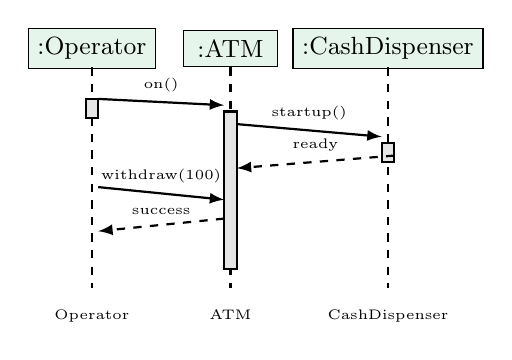
\begin{tikzpicture}[scale=0.8, every node/.style={font=\tiny}]
        % Object boxes
        \node[draw, rectangle, minimum width=1.2cm, minimum height=0.4cm, fill=tipbg] (op) at (0.8, 4) {\small :Operator};
        \node[draw, rectangle, minimum width=1.2cm, minimum height=0.4cm, fill=tipbg] (atm) at (3, 4) {\small :ATM};
        \node[draw, rectangle, minimum width=1.5cm, minimum height=0.4cm, fill=tipbg] (cash) at (5.5, 4) {\small :CashDispenser};
        
        % Lifelines
        \draw[dashed, thick] (0.8, 3.7) -- (0.8, 0.2);
        \draw[dashed, thick] (3, 3.7) -- (3, 0.2);
        \draw[dashed, thick] (5.5, 3.7) -- (5.5, 0.2);
        
        % Activation boxes
        \draw[fill=white!90!black, thick] (0.7, 3.2) rectangle (0.9, 2.9);
        \draw[fill=white!90!black, thick] (2.9, 3) rectangle (3.1, 0.5);
        \draw[fill=white!90!black, thick] (5.4, 2.5) rectangle (5.6, 2.2);
        
        % Messages
        \draw[-latex, thick] (0.9, 3.2) -- (2.9, 3.1) node[midway, above, font=\tiny] {on()};
        
        \draw[-latex, thick] (3.1, 2.8) -- (5.4, 2.6) node[midway, above, font=\tiny] {startup()};
        
        \draw[-latex, thick, dashed] (5.6, 2.3) -- (3.1, 2.1) node[midway, above, font=\tiny] {ready};
        
        \draw[-latex, thick] (0.9, 1.8) -- (2.9, 1.6) node[midway, above, font=\tiny] {withdraw(100)};
        
        \draw[-latex, thick, dashed] (2.9, 1.3) -- (0.9, 1.1) node[midway, above, font=\tiny] {success};
        
        % End points
        \node[font=\tiny, below] at (0.8, 0) {Operator};
        \node[font=\tiny, below] at (3, 0) {ATM};
        \node[font=\tiny, below] at (5.5, 0) {CashDispenser};
    \end{tikzpicture}
    \caption{Contoh Potongan Sequence Diagram Sistem ATM - Menunjukkan komunikasi antara Operator, ATM, dan CashDispenser dengan message flow (solid arrow) dan return value (dashed arrow).}
    \vspace{-0.3cm}
\end{figure}

Dengan Sequence Diagram, tim \textit{developer} bisa dengan sangat presisi melihat:
\begin{itemize}
    \item Urutan \textit{method} apa saja yang harus di-\textit{coding} dan dalam urutan apa
    \item Bagaimana pertukaran data antar kelas (objek) terjadi
    \item Parameter yang dibutuhkan dan nilai return yang diharapkan
    \item Sinkronisasi atau koordinasi antar objek yang kompleks
\end{itemize}

Sequence diagram menjadi blueprint yang sangat akurat untuk fase implementasi dan integration testing.

\end{document}
EOF
cat /home/claude/modul_uml_expanded.tex
Output

\documentclass[12pt,a4paper]{article}

% ─── 1. PACKAGES ──────────────────────────────────────────────────────────────
\usepackage[utf8]{inputenc}
\usepackage[T1]{fontenc}
\usepackage{amsmath, amssymb}
\usepackage{geometry}
\usepackage{graphicx}
\usepackage{xcolor}
\usepackage{listings}
\usepackage{hyperref}
\usepackage{booktabs}
\usepackage{enumitem}
\usepackage{tcolorbox}
\usepackage{mdframed}
\usepackage{fancyhdr}
\usepackage{titlesec}
\usepackage{tikz} 
\usetikzlibrary{shapes.geometric, positioning, arrows.meta, calc, trees}

% Font Settings
\usepackage{newtxtext,newtxmath} % Times New Roman
\usepackage{courier}             % Courier New untuk kode

\geometry{margin=2.5cm}

% ─── 2. WARNA TEMA ────────────────────────────────────────────────────────────
\definecolor{codebg}{RGB}{245,247,250}
\definecolor{codeframe}{RGB}{180,195,215}
\definecolor{keywordcolor}{RGB}{0,112,192}
\definecolor{commentcolor}{RGB}{100,160,100}
\definecolor{stringcolor}{RGB}{180,70,50}
\definecolor{notebg}{RGB}{255,249,230}
\definecolor{noteframe}{RGB}{230,180,50}
\definecolor{tipbg}{RGB}{230,245,235}
\definecolor{tipframe}{RGB}{50,160,90}
\definecolor{sectioncolor}{RGB}{30,80,150}

% ─── 3. STYLE SECTION & TOC ───────────────────────────────────────────────────
\titleformat{\section}{\Large\bfseries\color{sectioncolor}}{}{0em}{\thesection\quad}[\titlerule]
\titleformat{\subsection}{\large\bfseries\color{sectioncolor!80}}{}{0em}{\thesubsection\quad}

% Style Table of Contents
\usepackage{tocloft}
\renewcommand{\cftsecleader}{\cftdotfill{\cftdotsep}}
\renewcommand{\cftsecfont}{\bfseries\color{sectioncolor}}

% ─── 4. LISTINGS (CODE STYLE) ─────────────────────────────────────────────────
\lstdefinestyle{customstyle}{
  basicstyle=\ttfamily\small,
  backgroundcolor=\color{codebg},
  frame=single,
  rulecolor=\color{codeframe},
  keywordstyle=\bfseries\color{keywordcolor},
  commentstyle=\itshape\color{commentcolor},
  stringstyle=\color{stringcolor},
  numbers=left,
  numberstyle=\tiny\color{gray},
  breaklines=true,
  tabsize=4,
  showstringspaces=false
}
\lstset{style=customstyle}

% ─── 5. KOTAK CATATAN (MD-FRAME) ──────────────────────────────────────────────
\newmdenv[
  backgroundcolor=notebg, linecolor=noteframe, linewidth=2pt,
  leftline=true, topline=false, rightline=false, bottomline=false,
  innerleftmargin=10pt, innertopmargin=6pt, innerbottommargin=6pt, skipabove=8pt
]{notebox}

\newmdenv[
  backgroundcolor=tipbg, linecolor=tipframe, linewidth=2pt,
  leftline=true, topline=false, rightline=false, bottomline=false,
  innerleftmargin=10pt, innertopmargin=6pt, innerbottommargin=6pt, skipabove=8pt
]{tipbox}

% ─── 6. HEADER & FOOTER ───────────────────────────────────────────────────────
\pagestyle{fancy}
\fancyhf{}
\fancyhead[L]{\small\textit{Rekayasa Perangkat Lunak}}
\fancyhead[R]{\small\textit{noteify -- Pemodelan PL}}
\fancyfoot[C]{\thepage}
\renewcommand{\headrulewidth}{0.4pt}

% ─── 7. DATA COVER ────────────────────────────────────────────────────────────
\title{
  {\LARGE\bfseries REKAYASA PERANGKAT LUNAK}\\[0.5em]
  {\large Modul Pembelajaran: Pemodelan Perangkat Lunak dan UML}\\[0.8em]
  {\normalsize Penjelasan komprehensif mengenai konsep representasi sistem, landasan metodologi berorientasi objek, serta standar visualisasi diagram UML.}
}
\author{}
\date{}

% ==============================================================================
\begin{document}

\maketitle
\thispagestyle{fancy}
\tableofcontents
\newpage

% ─── KONTEN MATERI ─────────────────────────────────────────────────────────────

\section{Pemahaman Dasar Pemodelan Sistem}

Sebelum menulis baris kode program, seorang \textit{Software Engineer} harus mampu merancang cetak biru (\textit{blueprint}) dari sistem yang akan dibangun. Proses perancangan ini disebut dengan \textbf{pemodelan}.

Secara definisi, \textbf{Pemodelan (Model)} adalah representasi dari sebuah sistem nyata yang telah disederhanakan. Tujuannya agar kompleksitas sistem dapat lebih mudah dipelajari, dipahami, dan dikomunikasikan antar anggota tim. Dengan menggunakan model, tim pengembang dapat melakukan visualisasi, spesifikasi, konstruksi, dan dokumentasi secara lebih terstruktur sebelum sistem diimplementasikan dalam bentuk kode.

Ada 5 macam gaya atau cara merepresentasikan sebuah model sistem:

\begin{enumerate}
    \item \textbf{Physical (Fisik):} Membuat versi nyata dengan skala yang diperkecil (\textit{scaled-down version}) dari sistem yang dipelajari. Contohnya: miniatur model pesawat, model kereta api, atau prototipe hardware yang mendemonstrasikan aspek fungsional dari sistem sebenarnya.
    
    \item \textbf{Pictorial (Gambar):} Representasi menggunakan lukisan atau gambar untuk mendeskripsikan suatu bidang atau fenomena. Contohnya: peta topografi kontur bumi, bola dunia (globe), atau diagram aliran air dalam sistem hidrologi.
    
    \item \textbf{Verbal:} Representasi suatu sistem menggunakan susunan kata dan kalimat verbal yang mendeskripsikan ukuran, bentuk, dan karakteristik sistem tersebut. Pendekatan ini bermanfaat untuk dokumentasi requirements dan spesifikasi kebutuhan yang ditulis dalam bentuk narasi atau daftar kebutuhan.
    
    \item \textbf{Schematic (Skema):} Representasi dalam bentuk skema figuratif yang menggabungkan simbol-simbol dengan garis penghubung. Contohnya: skema rangkaian listrik, skema alur proses produksi, atau model atom Bohr dalam kimia.
    
    \item \textbf{Symbolic (Simbolik):} Representasi ke dalam bentuk simbol-simbol matematika, di mana karakteristik variabel diformulasikan menggunakan persamaan matematika. Pendekatan ini sangat berguna untuk sistem yang memiliki perilaku kuantitatif atau algoritma kompleks yang dapat diekspresikan secara matematis.
\end{enumerate}

\subsection{Karakteristik Kualitas Proses Pemodelan Analisis}

Saat melakukan proses pemodelan analisis, kita harus mengevaluasi apakah proses yang kita jalankan sudah baik atau belum. Evaluasi ini penting untuk memastikan bahwa model yang dihasilkan dapat digunakan secara efektif oleh seluruh tim pengembang. Ada 8 indikator kualitas proses analisis yang perlu dipertimbangkan:

\begin{itemize}
    \item \textbf{Understandability (Kemudahan Pemahaman):} Sejauh mana proses didefinisikan secara eksplisit dan seberapa mudah definisi proses itu dipahami oleh anggota tim. Model yang baik harus dapat dipahami oleh semua stakeholder tanpa memerlukan penjelasan yang berbelit-belit.
    
    \item \textbf{Visibility (Visibilitas):} Apakah aktivitas proses menghasilkan titik akhir (keluaran) yang jelas, sehingga kemajuan dari proses tersebut terlihat nyata. Setiap tahap harus menghasilkan deliverable yang terukur dan dapat diverifikasi.
    
    \item \textbf{Supportability (Dukungan Alat):} Sejauh mana aktivitas proses dapat didukung oleh alat bantu CASE (\textit{Computer-Aided Software Engineering}). Alat seperti ArchiMate, Enterprise Architect, atau Lucidchart dapat mempercepat proses pemodelan.
    
    \item \textbf{Acceptability (Penerimaan):} Apakah proses yang telah ditentukan dapat diterima, digunakan, dan dipertanggungjawabkan selama pembuatan perangkat lunak. Proses harus selaras dengan budaya organisasi dan tidak menimbulkan resistensi dari tim.
    
    \item \textbf{Reliability (Keandalan):} Apakah proses didesain sedemikian rupa sehingga \textit{error} (kesalahan) proses dapat dihindari sebelum merusak produk akhir. Mekanisme quality assurance dan review harus tertanam dalam proses.
    
    \item \textbf{Robustness (Ketangguhan):} Dapatkah proses pengembangan terus berjalan walaupun terjadi masalah \textit{error} yang tidak diduga di tengah jalan. Proses yang robust memiliki mekanisme fallback dan recovery yang baik.
    
    \item \textbf{Maintainability (Kemudahan Pemeliharaan):} Dapatkah proses berkembang dan beradaptasi untuk mengikuti perubahan kebutuhan atau perbaikan. Model dan proses harus mudah diperbarui tanpa memerlukan rekonstruksi total.
    
    \item \textbf{Rapidity (Kecepatan):} Bagaimana tingkat kecepatan proses untuk dapat memenuhi seluruh spesifikasi yang diminta secara lengkap. Proses yang baik harus efisien dalam hal waktu dan sumber daya tanpa mengorbankan kualitas.
\end{itemize}

\newpage
\section{Landskap Metodologi Analisis}

Secara garis besar, pendekatan pemodelan analisis terbagi menjadi dua mazhab besar: \textbf{Analisis Terstruktur} (klasik) dan \textbf{Analisis Berorientasi Objek} (modern). Analisis Terstruktur menggunakan pendekatan \textit{top-down} yang memecah sistem menjadi komponen-komponen data dan proses yang lebih kecil. Sebaliknya, Analisis Berorientasi Objek menggabungkan data dan perilaku ke dalam entitas yang disebut objek.

Pada modul ini, kita akan berfokus pada Metodologi Berorientasi Objek (\textit{Object-Oriented}). Sebelum standar UML diresmikan pada tahun 1997, ada banyak pakar yang menciptakan metode \textit{Object-Oriented} (OO) mereka sendiri dengan notasi dan terminologi yang berbeda-beda. Berikut adalah 6 metode OO paling bersejarah yang akhirnya melebur menjadi UML:

\begin{enumerate}
    \item \textbf{Metode Booch (Object Oriented Design)}\\
    Metode ini dikembangkan oleh Grady Booch dan membagi proses analisis dan desain ke dalam 4 tahapan iteratif (berulang): 
    \begin{enumerate}[label=(\arabic*)]
        \item Identifikasi kelas dan objek dari domain masalah
        \item Identifikasi semantik dan hubungan antar objek
        \item Perincian \textit{interface} (antarmuka) dan implementasi
        \item Dokumentasi dan verifikasi
    \end{enumerate}
    Metode ini terkenal dengan diagram object-oriented yang detail dan notation yang comprehensive.
    
    \item \textbf{Metode Rumbaugh (Object Modelling Technique - OMT)}\\
    Berdasarkan pada analisis terstruktur dan pemodelan \textit{Entity Relationship} (ER). Memiliki 3 tahap utama: 
    \begin{enumerate}[label=(\arabic*)]
        \item Analisis Object Model, Dynamic Model, dan Functional Model
        \item Desain Sistem dan desain Object-oriented
        \item Implementasi dan pengujian
    \end{enumerate}
    Keunggulannya adalah memiliki notasi yang mendukung semua konsep OO dan mudah diterapkan oleh tim yang sudah terbiasa dengan ER diagram.
    
    \item \textbf{Metode Jacobson (Object Oriented Software Engineering - OOSE)}\\
    Metode inilah yang menjadi cikal bakal (pioneer) konsep \textit{Use-Case} yang sangat popular hingga saat ini. Tahapannya meliputi: 
    \begin{enumerate}[label=(\arabic*)]
        \item Model \textit{requirement} dan analisis menggunakan use-case
        \item Desain dan implementasi architecture
        \item Model pengujian (test model)
    \end{enumerate}
    Keunggulannya adalah notasinya sangat sederhana, mudah dipelajari, dan sangat efektif untuk komunikasi dengan stakeholder non-teknis.
    
    \item \textbf{Metode Coad dan Yourdon}\\
    Berfokus pada pemodelan OO dan ER dengan 4 komponen perancangan: 
    \begin{enumerate}[label=(\arabic*)]
        \item Problem domain (domain masalah)
        \item Human interaction (interaksi manusia / UI)
        \item Data management (manajemen data / persistence)
        \item Task management (manajemen tugas / workflow)
    \end{enumerate}
    Metode ini sangat aplikatif untuk sistem bisnis yang kompleks.
    
    \item \textbf{Metode Wirfs-Brock (RDD / CRC - Responsibility Driven Design)}\\
    Metode \textit{Responsibility Driven Design} (RDD) ini sangat berguna untuk memunculkan ide di tahap awal analisis. Metode ini menggunakan kartu CRC (\textit{Class Responsibility Collaboration}) untuk mengidentifikasi:
    \begin{enumerate}[label=(\arabic*)]
        \item Kelas dan tanggung jawab (responsibility) masing-masing
        \item Kolaborasi antar kelas
        \item Hierarki pewarisan kelas
    \end{enumerate}
    Pendekatan ini sangat interaktif dan sering digunakan dalam workshop analisis kelompok.
    
    \item \textbf{Metode Shlaer-Mellor (OOA/D Tradisional)}\\
    Menghasilkan tiga jenis model yang saling melengkapi:
    \begin{enumerate}[label=(\arabic*)]
        \item Information model (diagram class/entity)
        \item State model (diagram state/transisi state)
        \item Process model (diagram aksi dan aktivitas)
    \end{enumerate}
    Metode ini sangat mudah dikonversi dari metode struktural lama ke OO, sehingga cocok untuk organisasi yang sedang melakukan transisi dari structured programming ke object-oriented.
\end{enumerate}

\newpage
\section{Pengenalan Unified Modeling Language (UML)}

Karena dulu banyak pakar yang membuat standar diagramnya sendiri-sendiri, masing-masing dengan kelebihan dan kelemahan tersendiri, akhirnya pada pertengahan 1990-an disepakatilah sebuah standar global yang menggabungkan praktik terbaik dari semua metode di atas. Standar tersebut bernama \textbf{Unified Modeling Language (UML)}, yang diresmikan oleh \textit{Object Management Group (OMG)} pada tahun 1997.

UML adalah kumpulan notasi yang lengkap untuk membuat visualisasi model suatu sistem. Notasi-notasi ini bersifat grafis dan memiliki semantik yang jelas, sehingga dapat dipahami oleh berbagai stakeholder. Tujuan utama diciptakannya UML adalah:

\begin{enumerate}
    \item Memberikan bahasa pemodelan visual yang ekspresif, siap pakai, dan mudah dimengerti secara umum agar pengembang dapat saling menukar model dan berkomunikasi dengan efektif.
    
    \item Memberikan standar pemodelan yang independen (bebas dari ikatan bahasa pemrograman tertentu, platform tertentu, atau proses rekayasa tertentu), sehingga UML dapat diterapkan di berbagai konteks dan lingkungan.
    
    \item Menyatukan \textit{best-practices} (praktik-praktik terbaik) yang selama ini digunakan dalam dunia pemodelan sistem, menciptakan satu bahasa bersama untuk industri software engineering.
\end{enumerate}

\subsection{Kategori Diagram dalam UML}

Ada beberapa jenis diagram utama dalam UML yang dapat dikelompokkan berdasarkan fungsinya:

\begin{itemize}
    \item \textbf{Diagram Struktur (Structural Diagrams):} Menggambarkan elemen-elemen statis dalam sistem seperti kelas, objek, komponen, dan hubungan antar mereka. Termasuk: Class Diagram, Object Diagram, Component Diagram, Deployment Diagram, Package Diagram.
    
    \item \textbf{Diagram Perilaku (Behavioral Diagrams):} Menggambarkan aspek dinamis atau perilaku sistem, bagaimana sistem berinteraksi dan bereaksi terhadap events. Termasuk: Use Case Diagram, Sequence Diagram, Activity Diagram, State Machine Diagram, Communication Diagram, Interaction Overview Diagram.
\end{itemize}

Mari kita bahas beberapa diagram utama secara mendetail.

\newpage
\section{1. Use Case Diagram}

\textbf{Use Case Diagram} merupakan sebuah diagram yang bertujuan untuk menggambarkan \textbf{fungsionalitas} (feature atau capability) yang diharapkan dari sebuah sistem. Diagram ini fokus mendeskripsikan interaksi atau hubungan antara \textit{Aktor} (pengguna/pihak luar) dengan \textit{Sistem} itu sendiri melalui sebuah skenario cerita penggunaan (use case).

Use Case Diagram sangat bermanfaat pada tahap awal analisis kebutuhan (\textit{requirements analysis}) karena:
\begin{itemize}
    \item Membantu mengidentifikasi semua pengguna sistem (aktor) dan kebutuhan mereka
    \item Memberikan gambaran high-level tentang apa yang bisa dilakukan sistem
    \item Memfasilitasi komunikasi antara developer dan stakeholder
    \item Menjadi dasar untuk pembuatan test cases dan dokumentasi kebutuhan
\end{itemize}

Ada 6 elemen/komponen pembentuk Use Case Diagram:

\textbf{1. System (Sistem)}\\
Menyatakan batasan (\textit{boundary}) ruang lingkup sistem. Digambarkan dengan kotak segi empat yang membatasi semua use case di dalamnya. Semua aktor harus berada di luar kotak ini. (Catatan: Seringkali kotak batas sistem ini disembunyikan/tidak digambar karena dianggap sudah jelas dari konteks).

\textbf{2. Actor (Aktor)}\\
Aktor adalah entitas di luar sistem yang akan menggunakan atau berinteraksi dengan sistem tersebut. Aktor tidak selalu manusia; ia bisa berupa \textit{device} (perangkat keras seperti sensor, printer) atau bahkan sistem/server lain (seperti database server, payment gateway). Cara mudah mencari aktor adalah dengan bertanya: \textit{``Siapa/apa yang akan menggunakan sistem ini?''} dan \textit{``Apakah sistem ini memberikan nilai/manfaat bagi dia?''} Setiap aktor dalam diagram harus mempunyai setidaknya satu use case.

\textbf{3. Use Case (Fungsionalitas)}\\
Mengidentifikasi fitur atau \textit{goal} (tujuan) utama dari sistem yang dicapai melalui interaksi dengan aktor. Digambarkan dengan bentuk Elips oval dengan nama aktivitas di dalamnya. Setiap use case pasti memiliki pemicu (\textit{trigger}) yang memulainya. \textit{Trigger} bisa bersifat \textbf{eksternal} (misal: user menekan tombol pesan) atau \textbf{temporal/waktu} (misal: alarm berbunyi saat jadwal jatuh tempo).

\textbf{4. Association (Asosiasi)}\\
Garis penghubung yang mengidentifikasi interaksi antara aktor dengan use case tertentu. Bisa berupa garis lurus tanpa panah (interaksi dua arah) atau dengan panah (komunikasi satu arah). Association mewakili partisipasi dari aktor dalam use case tersebut.

\textbf{5. Dependency (Ketergantungan)}\\
Garis putus-putus berpanah yang menunjukkan hubungan ketergantungan antar dua Use Case. Terdiri dari 2 jenis:
\begin{itemize}
    \item \textbf{<<include>> (Inclusion):} Use case yang satu WAJIB memanggil use case yang lain agar bisa selesai dengan sempurna. Hubungan ini bersifat unconditional dan mandatory. (Arah panah menuju ke use case yang dipanggil/included).
    \item \textbf{<<extend>> (Extension):} Pemanggilan use case tambahan HANYA JIKA kondisi tertentu terpenuhi (opsional). Hubungan ini bersifat conditional dan optional. (Arah panah berlawanan, menuju ke use case pemanggil/yang diperluas).
\end{itemize}

\textbf{6. Generalization (Generalisasi)}\\
Mendefinisikan relasi pewarisan sifat (\textit{inheritance}) antar use case atau antar aktor. Digambarkan dengan garis bermata panah kosong (segitiga putih) yang mengarah dari sisi \textit{Child} (anak) ke sisi \textit{Parent} (induk). Ini menunjukkan bahwa aktor child mewarisi semua karakteristik dari parent.

\begin{figure}[h]
    \centering
    \vspace{-0.5cm}
    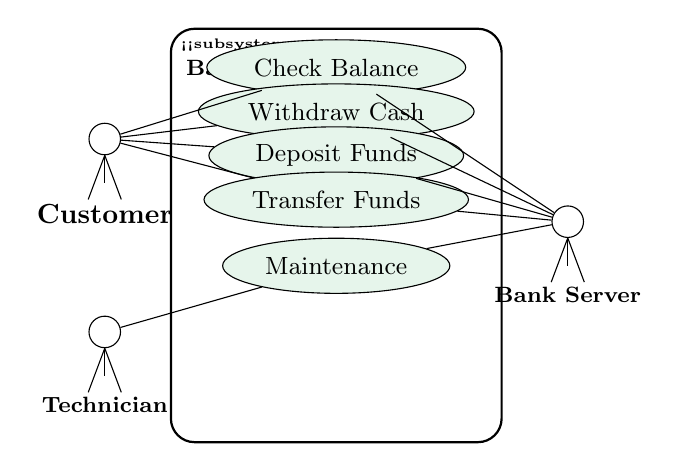
\begin{tikzpicture}[scale=0.7, every node/.style={font=\small}]
    
        % System Boundary
        \draw[thick, rounded corners=0.3cm] (1.5, 3.5) rectangle (7.5, -4);
        \node[anchor=north west, font=\tiny] at (1.5, 3.5) {\textbf{<<subsystem>>}};
        \node[anchor=north west, font=\footnotesize\bfseries] at (1.6, 3.1) {Bank ATM};
        
        % Actors - Left side (Customer)
        \node[draw, circle, minimum size=0.4cm, inner sep=0] (cust) at (0.3, 1.5) {};
        \draw (cust.south) -- ++(0, -0.5);
        \draw (cust.south) -- ++(-0.3, -0.8);
        \draw (cust.south) -- ++(0.3, -0.8);
        \node[below=0.5cm of cust, font=\footnotesize, font=\bfseries] {Customer};
        
        % Actors - Left side (Technician)
        \node[draw, circle, minimum size=0.4cm, inner sep=0] (tech) at (0.3, -2) {};
        \draw (tech.south) -- ++(0, -0.5);
        \draw (tech.south) -- ++(-0.3, -0.8);
        \draw (tech.south) -- ++(0.3, -0.8);
        \node[below=0.5cm of tech, font=\footnotesize\bfseries] {Technician};
        
        % Actors - Right side (Bank)
        \node[draw, circle, minimum size=0.4cm, inner sep=0] (bank) at (8.7, 0) {};
        \draw (bank.south) -- ++(0, -0.5);
        \draw (bank.south) -- ++(-0.3, -0.8);
        \draw (bank.south) -- ++(0.3, -0.8);
        \node[below=0.5cm of bank, font=\footnotesize\bfseries] {Bank Server};
        
        % Use Cases
        \node[draw, ellipse, minimum width=2cm, minimum height=0.7cm, fill=tipbg] (uc1) at (4.5, 2.8) {\small Check Balance};
        \node[draw, ellipse, minimum width=2cm, minimum height=0.7cm, fill=tipbg] (uc2) at (4.5, 2) {\small Withdraw Cash};
        \node[draw, ellipse, minimum width=2cm, minimum height=0.7cm, fill=tipbg] (uc3) at (4.5, 1.2) {\small Deposit Funds};
        \node[draw, ellipse, minimum width=2cm, minimum height=0.7cm, fill=tipbg] (uc4) at (4.5, 0.4) {\small Transfer Funds};
        \node[draw, ellipse, minimum width=2cm, minimum height=0.7cm, fill=tipbg] (uc5) at (4.5, -0.8) {\small Maintenance};
        
        % Associations
        \draw (cust) -- (uc1);
        \draw (cust) -- (uc2);
        \draw (cust) -- (uc3);
        \draw (cust) -- (uc4);
        \draw (tech) -- (uc5);
        
        % Associations with Bank Server
        \draw (uc1) -- (bank);
        \draw (uc2) -- (bank);
        \draw (uc3) -- (bank);
        \draw (uc4) -- (bank);
        \draw (uc5) -- (bank);
    \end{tikzpicture}
    \caption{Contoh Use Case Diagram Sistem Bank ATM - Menunjukkan aktor (Customer, Technician, Bank Server) dan use case (Check Balance, Withdraw Cash, dll) dengan asosiasi dan batasan sistem.}
    \vspace{-0.3cm}
\end{figure}

\newpage
\section{2. Activity Diagram}

Jika Use Case fokus pada \textbf{``Apa''} yang bisa dilakukan sistem, \textbf{Activity Diagram} berfokus pada \textbf{``Bagaimana''} alur kerja (\textit{workflow}) dan proses bisnis sistem tersebut secara rinci. Activity diagram menampilkan urutan (sequence) dari aktivitas-aktivitas, keputusan-keputusan (decision points), dan sinkronisasi (synchronization) antar aktivitas.

Activity diagram menggambarkan berbagai alur aktivitas dalam sistem:
\begin{itemize}
    \item Bagaimana masing-masing alur berawal (starting point)
    \item Pengambilan keputusan (\textit{decision}) yang mungkin terjadi dan kondisi-kondisinya
    \item Bagaimana alur tersebut berakhir (ending point)
    \item Aktivitas yang berjalan paralel atau bersamaan (\textit{concurrent activities})
    \item Objek atau data yang mengalir dari satu aktivitas ke aktivitas lain
\end{itemize}

Perlu dipahami bahwa Activity Diagram ini tidak menggambarkan \textit{behaviour} (perilaku) eksak internal antar subsistem, melainkan lebih ke gambaran proses bisnis level atas secara umum. Oleh karena itu, Activity Diagram sangat cocok untuk komunikasi dengan non-technical stakeholder seperti business analyst atau user.

\subsection{Simbol-Simbol Activity Diagram}

Terdapat beberapa notasi simbol standar yang harus digunakan dalam activity diagram:

\begin{table}[h]
\centering
\begin{tabular}{@{}p{3cm}p{10.5cm}@{}}
\toprule
\textbf{Nama Simbol} & \textbf{Keterangan / Fungsi} \\ \midrule
\textbf{Action/Activity} & Digambarkan dengan kotak dengan sudut yang membulat (\textit{rounded rectangle}). Merupakan state yang mencerminkan eksekusi dari suatu aksi atau pekerjaan konkret. Contoh: ``Proses Pembayaran'', ``Update Database''. \\ \addlinespace
\textbf{Initial Node} & Titik hitam bulat penuh (filled circle). Menandakan bagaimana aktivitas sistem bermula atau dimulai (Start point). Setiap diagram harus memiliki exactly satu initial node. \\ \addlinespace
\textbf{Final Node} & Titik hitam dengan lingkaran luar (target symbol). Menandakan bagaimana aktivitas sistem diakhiri secara keseluruhan (End point). Diagram dapat memiliki multiple final nodes untuk berbagai skenario akhir. \\ \addlinespace
\textbf{Decision} & Bentuk belah ketupat (\textit{diamond}). Digunakan untuk menggambarkan suatu keputusan atau tindakan bercabang yang harus diambil pada kondisi tertentu (IF-ELSE logic). Edge yang keluar dari decision harus memiliki label kondisi (guard condition). \\ \addlinespace
\textbf{Merge} & Bentuk belah ketupat dengan multiple edge input tapi single output. Digunakan untuk menggabungkan beberapa alur menjadi satu setelah decision point. Berbeda dengan decision yang membagi alur. \\ \addlinespace
\textbf{Fork/Join Bar} & Garis horizontal tebal. Fork memisahkan satu alur menjadi beberapa alur paralel yang berjalan bersamaan. Join menggabungkan beberapa alur paralel menjadi satu dan menunggu semua alur selesai. \\ \addlinespace
\textbf{Control Flow} & Garis panah yang menghubungkan satu simbol aktivitas ke simbol lainnya sesuai urutan eksekusi. Label pada garis dapat menunjukkan kondisi atau event. \\ \bottomrule
\end{tabular}
\end{table}

\subsection{Swimlane dalam Activity Diagram}

Fitur penting lainnya di Activity Diagram adalah \textbf{Swimlane} (juga disebut \textit{partition}). \textit{Swimlane} ini membagi area diagram ke dalam beberapa partisi kolom (mirip jalur renang dalam kolam renang) yang mewakili entitas, aktor, atau departemen mana yang sedang bertanggung jawab melakukan suatu aktivitas pada saat itu. Dengan swimlane, kita dapat dengan jelas melihat siapa responsible untuk apa, sehingga sangat berguna untuk menunjukkan ownership dan accountability dalam proses bisnis. Swimlane dapat diatur secara horizontal (vertical partitions untuk aktor) atau vertikal (horizontal partitions untuk organizational units).

\newpage
\section{3. Sequence Diagram}

\textbf{Sequence Diagram} adalah diagram yang sangat teknis dan detail. Diagram ini menggambarkan interaksi antara objek-objek (atau komponen-komponen) di dalam dan di sekitar sistem. Interaksi ini mencakup pengguna (actor), antarmuka pengguna (UI), pengontrol (controller), logika bisnis (business logic), dan database. Sequence diagram memperlihatkan urutan waktu dari setiap message (pesan) yang dikirim dan diterima.

Karakteristik utama Sequence Diagram adalah:

\begin{itemize}
    \item Menggambarkan interaksi berupa \textbf{pesan (\textit{message})} yang dikirim dan diterima antar objek. Pesan dapat berupa method call, return value, atau event.
    
    \item Interaksi ini dipetakan secara terstruktur \textbf{terhadap waktu}. Waktu mengalir dari atas ke bawah, sehingga event yang lebih atas terjadi lebih dulu.
    
    \item Terdiri atas dua dimensi utama: 
    \begin{enumerate}[label=(\arabic*)]
        \item \textbf{Dimensi Vertikal} yang mewakili aliran waktu (semakin ke bawah = semakin akhir dalam timeline)
        \item \textbf{Dimensi Horizontal} yang mewakili objek-objek yang sedang saling berkomunikasi
    \end{enumerate}
\end{itemize}

Sequence diagram sangat berguna karena:
\begin{itemize}
    \item Menunjukkan detail alur eksekusi dari setiap use case
    \item Membantu tim developer memahami urutan method call dan data flow
    \item Mengidentifikasi potential issues seperti deadlock atau race condition
    \item Menjadi blueprint untuk implementasi kode
\end{itemize}

\subsection{Simbol-Simbol Sequence Diagram}

Elemen pembentuk diagram ini antara lain:

\begin{table}[h]
\centering
\begin{tabular}{@{}p{3.5cm}p{10cm}@{}}
\toprule
\textbf{Nama Simbol} & \textbf{Keterangan / Fungsi} \\ \midrule
\textbf{Actor/Object Box} & Kotak header di bagian atas diagram yang merepresentasikan aktor atau objek. Dituliskan dengan format \texttt{objectName : ClassName}. \\ \addlinespace
\textbf{LifeLine} & Garis vertikal putus-putus yang membentang ke bawah dari setiap object box. Menggambarkan eksistensi atau periode hidup dari objek, entitas, atau antarmuka tersebut selama waktu tertentu. \\ \addlinespace
\textbf{Message} & Garis panah horizontal penuh (solid arrow). Spesifikasi komunikasi antar objek yang memuat aksi, pemanggilan fungsi (\textit{method}), atau perintah yang dieksekusi oleh objek tujuan. Dapat memiliki parameter dan return type. \\ \addlinespace
\textbf{Return Message} & Garis panah horizontal putus-putus (dashed arrow). Menandakan nilai kembalian atau respon balasan dari objek yang dipanggil kembali ke objek pemanggil. Dapat disertai dengan nilai return. \\ \addlinespace
\textbf{Activation Box} & Kotak vertikal tipis pada lifeline yang menunjukkan periode waktu ketika objek sedang aktif (melakukan pekerjaan atau menunggu response). Dimulai saat method dipanggil dan berakhir saat method selesai/return. \\ \addlinespace
\textbf{Alt/Opt/Loop Frame} & Kotak interaksi besar yang membungkus beberapa message untuk menunjukkan conditional logic (\textit{Alt}), optional behavior (\textit{Opt}), atau repeated behavior (\textit{Loop}). \\ \bottomrule
\end{tabular}
\end{table}

\begin{figure}[h]
    \centering
    \vspace{-0.5cm}
    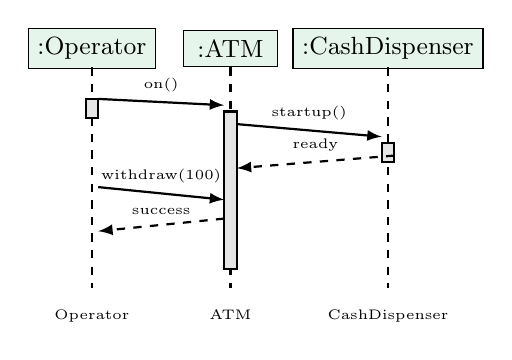
\begin{tikzpicture}[scale=0.8, every node/.style={font=\tiny}]
        % Object boxes
        \node[draw, rectangle, minimum width=1.2cm, minimum height=0.4cm, fill=tipbg] (op) at (0.8, 4) {\small :Operator};
        \node[draw, rectangle, minimum width=1.2cm, minimum height=0.4cm, fill=tipbg] (atm) at (3, 4) {\small :ATM};
        \node[draw, rectangle, minimum width=1.5cm, minimum height=0.4cm, fill=tipbg] (cash) at (5.5, 4) {\small :CashDispenser};
        
        % Lifelines
        \draw[dashed, thick] (0.8, 3.7) -- (0.8, 0.2);
        \draw[dashed, thick] (3, 3.7) -- (3, 0.2);
        \draw[dashed, thick] (5.5, 3.7) -- (5.5, 0.2);
        
        % Activation boxes
        \draw[fill=white!90!black, thick] (0.7, 3.2) rectangle (0.9, 2.9);
        \draw[fill=white!90!black, thick] (2.9, 3) rectangle (3.1, 0.5);
        \draw[fill=white!90!black, thick] (5.4, 2.5) rectangle (5.6, 2.2);
        
        % Messages
        \draw[-latex, thick] (0.9, 3.2) -- (2.9, 3.1) node[midway, above, font=\tiny] {on()};
        
        \draw[-latex, thick] (3.1, 2.8) -- (5.4, 2.6) node[midway, above, font=\tiny] {startup()};
        
        \draw[-latex, thick, dashed] (5.6, 2.3) -- (3.1, 2.1) node[midway, above, font=\tiny] {ready};
        
        \draw[-latex, thick] (0.9, 1.8) -- (2.9, 1.6) node[midway, above, font=\tiny] {withdraw(100)};
        
        \draw[-latex, thick, dashed] (2.9, 1.3) -- (0.9, 1.1) node[midway, above, font=\tiny] {success};
        
        % End points
        \node[font=\tiny, below] at (0.8, 0) {Operator};
        \node[font=\tiny, below] at (3, 0) {ATM};
        \node[font=\tiny, below] at (5.5, 0) {CashDispenser};
    \end{tikzpicture}
    \caption{Contoh Potongan Sequence Diagram Sistem ATM - Menunjukkan komunikasi antara Operator, ATM, dan CashDispenser dengan message flow (solid arrow) dan return value (dashed arrow).}
    \vspace{-0.3cm}
\end{figure}

Dengan Sequence Diagram, tim \textit{developer} bisa dengan sangat presisi melihat:
\begin{itemize}
    \item Urutan \textit{method} apa saja yang harus di-\textit{coding} dan dalam urutan apa
    \item Bagaimana pertukaran data antar kelas (objek) terjadi
    \item Parameter yang dibutuhkan dan nilai return yang diharapkan
    \item Sinkronisasi atau koordinasi antar objek yang kompleks
\end{itemize}

Sequence diagram menjadi blueprint yang sangat akurat untuk fase implementasi dan integration testing.

\end{document}